\section{Описание практической части}
\label{sec:Chapter4} \index{Chapter4}

\subsection{Использованные инструменты}

В данном разделе будет приведен список инструментов, используемых в ходе практической части работы.

В ходе всей работы по тестированию JFFS2 используется код ядра Linux версии 5.10 из репозитория \cite{lvcrepo} лаборатории Linux Verification Center. Процесс тестирования происходит на виртуальной машине Qemu, эмулирующей машину архитектуры x86-64 под гостевой системой Ubuntu Linux.

Для тестирования сценариев работы с различными типами устройств флэш-памяти без использования реальных микросхем памяти, необходимо использовать эмуляторы флэш-устройств. На данный момент в модуле устройств на основе технологии памяти (MTD) \cite{mtd} ядра Linux реализованы 3 эмулятора: mtdram, эмулирующий NOR-память в оперативной памяти системы, block2mtd, эмулирующий устройство NOR-памяти поверх блочного устройства и nandsim, эмулирующий устройство NAND-памяти в оперативной памяти. Поддержка эмуляторов подключается в файле конфигурации ядра, например, параметр "CONFIG\_MTD\_MTDRAM"\ отвечает за использование эмулятор mtdram, а параметры "CONFIG\_MTDRAM\ \_TOTAL\_SIZE"\ и "CONFIG\_MTDRAM\_ERASE\_SIZE"\ устанавливают размер эмулируемого устройства и размер его стираемого блока.

За основу при создании системы автоматизированного тестирования было решено взять тестовый набор xfstests, так как он содержит в себе множество скриптов, тестирующих базовые функции, общие для всех ФС, а также является наиболее популярным решением для тестирования файловых систем ядра Linux и имеет удобный функционал для добавления новых тестов. Для добавления в набор xfstests своих тестовых сценариев необходимо описать сценарий в виде bash-скрипта, запустить скрипт new для добавления нового теста в набор и создать файл, определяющий выходные данные, которые должны генерироваться в ходе корректной работы теста. При тестировании xfstests использует 2 блочных устройства, называющиеся TEST и SCRATCH с тестируемой ФС на них и два каталога, используемые для монтирования. Для предоставления тестовому набору интерфейса блочного устройства в модуле MTD есть драйвер mtdblock. Для использования этого драйвера необходимо установить соответствующую ему опцию конфигурации ядра, что делается при помощи строки  "CONFIG\_MTD\_BLOCK=y".

Для сбора информации о покрытии исходного кода модулей ядра используется утилита gcov \cite{gcov}. Для визуализации собранной информации в виде html отчета используется расширение утилиты gcov - lcov \cite{lcov}. Для сбора информации о покрытии в ядре Linux достаточно установить параметр конфигурации ядра "CONFIG\_GCOV\_KERNEL"\ при его сборке, а так же параметр "GCOV\_PROFILE"\ в файле сборки модуля fs/jffs2/Makefile для активации профилирования директории,содержащей исходные файлы тестируемой ФС. Для сбора корректного покрытия в ходе работы тестов перед запуском необходимо сбросить информацию о покрытии. Сброс покрытия можно осуществить командой  "echo 0 > /sys/kernel/debug/gcov/reset". После окончания работы тестов, информация о покрытии хранится в директории /sys/kernel/debug/gcov. На основе собранного покрытия утилита lcov генерирует информационный файл, который преобразуется в html-отчет утилитой genhtml. Пример отчета о собранном покрытии представлен на рис. \ref{coverexample}

\begin{figure}[H]
	\centering
	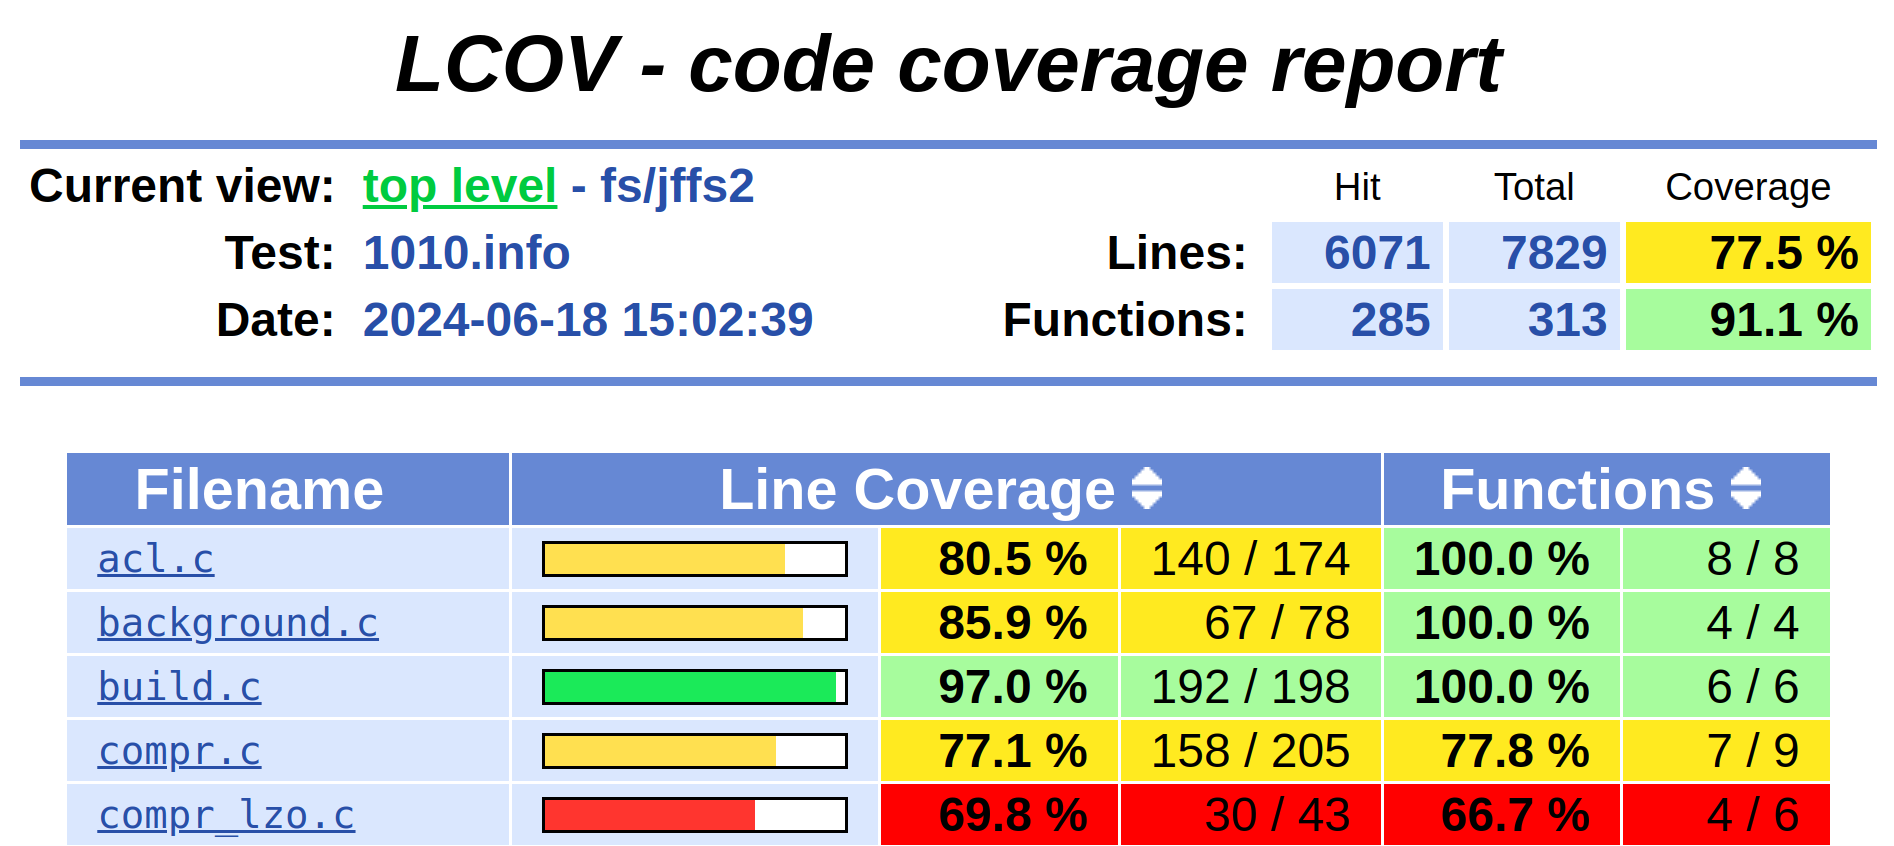
\includegraphics[scale=0.2]{cover-ex.png}
	\caption{HTML отчет о покрытии, сгенерированный утилитой genhtml.}
	\label{coverexample}
\end{figure}

Для создания тестируемого образа файловой системы используется команда mkfs с опцией определяющей тип файловой системы. Команда для создания образа JFFS2 (mkfs.jffs2) является частью пакета инструментов для работы с флэш-памятью mtd-utils \cite{mtd-utils}. По неизвестной причине, из четырех алгоритмов сжатия, поддерживаемых JFFS2, команда создания образа файловой системы поддерживала только 3: lzo, zlib и rtime. С целью достичь более полного тестирования исходного кода, в процессе работы исходный код инструмента mkfs.jffs2 был доработан, и таким образом была добавлена возможность создания образа JFFS2 с использованием алгоритма сжатия rubin.

Как было описано в прошлой главе, JFFS2 имеет специальные функции для работы с устройствами dataflash, подключенными по протоколу SPI и устройствами разделенными на томы с несортированными блоками (UBI устройства) \cite{ubi}. К сожалению в открытом доступе нет эмулятора устройства dataflash, для тестирования сценария монтирования устройства такого типа, однако в модуле MTD есть эмулятор устройств с несортированными блоками - gluebi. Для подключения этого эмулятора в конфигурационном файле ядра используется строка "CONFIG\_MTD\_UBI\_GLUEBI=y". Подсистема UBI, являющаяся частью модуля MTD выполняет функции уровня флэш-преобразования, обеспечивая выравнивание износа блоков устройства, а также управляет томами, являющимися более высокоуровневой абстракцией над устройствами технологии памяти. В процессе практической работы, эмулятор gluebi вызывал панику ядра путем разыменования нулевого указателя. Для корректного использования эмулятора потребовалось исправление его исходного кода.

Для покрытия функций обработки ошибок фаззинг-тестированием, в работе будут использованы инструменты syzkaller \cite{syzkaller} и fsfuzz \cite{fsfuzz}. Не смотря на то, что в документации инструмент фаззинг-тестирования файловых систем fsfuzz заявляется о совместимости с файловой системой JFFS2, прямолинейный запуск инструмента для исследуемой ФС не принес результата, так как bash-скрипт fsfuzz использует при монтировании виртуальные блочные устройства, что является неподходящим для JFFS2. После внесения правок в исходный код инструмента с целью использования MTD устройств при указании в качестве опции тип файловой системы JFFS2, инструмент удалось применить к тестированию исследуемой ФС.

Для симуляции сбоев во внутренних функциях модуля ФС в работе будет применен встроенный в ядро Linux инструмент Linux Fault Injection \cite{fault}. Этот инструмент позволяет симулировать сбои почти всех функций ядра, предоставляя пользователю возможность установить в качестве параметров вероятность ошибки, интервал между сбоями, их количество и возвращаемое функцией значение. Для симуляции сбоя функции необходимо разрешить в коде ядра внедрение неисправности в эту функцию при помощи макроса ALLOW\_ERROR\_INJECTION. Сам инструмент можно использовать при установке параметра конфигурации ядра "CONFIG\_ FAULT\_INJECTION".

\subsection{Тестирование с использованием готовых решений}

Для тестирования файловой системы с использованием готовых решений необходима предварительная сборка ядра с определенной конфигурацией, наличие тестируемого образа файловой системы и блочных устройств для монтирования. Далее в этом разделе будет описана базовая конфигурация, необходимая для тестирования JFFS2 при помощи готовых решений.

Во первых, необходимо в конфигурации ядра добавить поддержку тестируемой ФС и необходимой для ее работы подсистемы устройств технологии памяти, которая отсутствует в базовой конфигурации ядра. Это может быть осуществлено добавлением следующих строк в файл конфигурации ядра Linux: "CONFIG\_MTD=y"\ - подключение подсистемы MTD, "CONFIG\_JFFS2\_FS=y"\ - подключение модуля JFFS2. Во-вторых, после конфигурации и сборки ядра необходимо создать образ тестируемой ФС. Для этого используется команда mkfs.jffs2, являющаяся частью пакета инструментов mtd-utils, который требует предварительной установки, например, при помощи менеджера пакетов apt-get. В третьих, для монтирования тестируемой ФС необходимы блочные устройства, которые в случае JFFS2 создаются драйвером mtdblock поверх MTD устройств эмулируемых одним из эмуляторов, например, block2mtd, который тоже необходимо подключить в конфигурации ядра.

\subsection{Результаты первого эксперимента}

Прямолинейный запуск набора xfstests в совокупности с тестами из пакета mtd-utils в описаной выше минимальной необходимой конфигурации дал результат в виде тестового покрытия исходного кода в 64\% исходного кода. 

\begin{figure}[H]
	\centering
	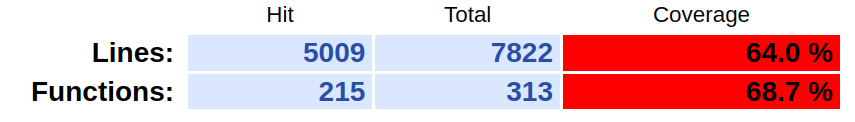
\includegraphics[scale=0.5]{cover1.png}
	\caption{Результат первого эксперимента}
	\label{cover1}
\end{figure} 

Следующим важным шагом является расширение тестового покрытия, на основе анализа функционала JFFS2 и параметров окружения, который был приведен в прошлой главе, а также анализа достигнутого в первом эксперименте покрытия. 

\subsection{Расширение тестового покрытия}

Первым шагом на пути к расширению тестового покрытия является добавление в конфигурации ядра всего функционала тестируемой ФС. Опции конфигурации JFFS2 и функционал на который они влияют описаны в файле fs/jffs2/Kconfig. Опции конфигурации и их назначение описаны в таблице на рис. ~\ref{table1}.

\begin{figure}[H]
	\centering
	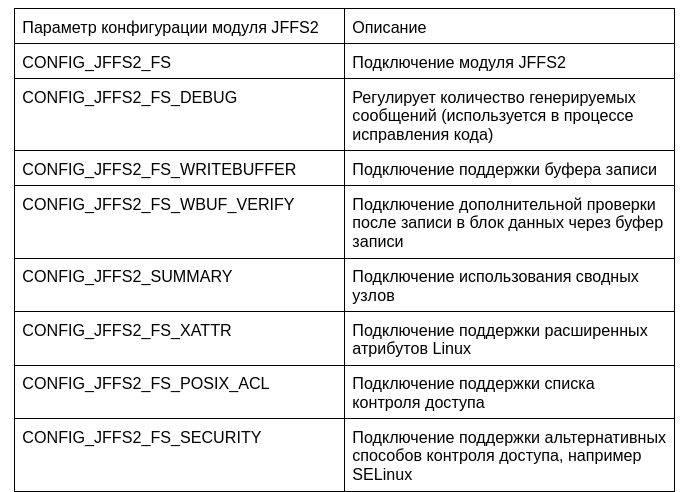
\includegraphics[scale=0.5]{table1.png}
	\caption{Опции конфигурации ядра для сборки модуля JFFS2}
	\label{table1}
\end{figure}

Анализ достигнутого при первом эксперименте покрытия показал, что не покрыты функции, используемые для работы с устройствами NAND-памяти и UBI томами, так как используемые эмулятор block2mtd эмулирован флэш-память NOR-типа. Для расширения тестового покрытия необходимо использовать эмулятор UBI томов gluebi и NAND-памяти nandsim.

\begin{figure}[H]
	\centering
	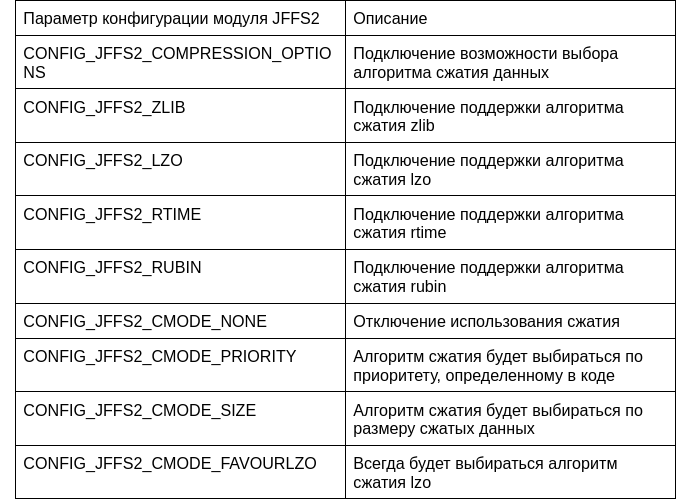
\includegraphics[scale=0.5]{table2.png}
	\caption{Опции конфигурации ядра для сборки модуля JFFS2 (Продолжение)}
	\label{table2}
\end{figure}

Также не были покрыты функции алгоритмов сжатия данных. Для их покрытия необходимо подключить их поддержку в конфигурации ядра, создать несколько тестируемых образов с разными параметрами mkfs, например, команда "mkfs.jffs2 \-\-compression-mode=size"\ создает образ ФС, алгоритм сжатия на котором будет определяться размерам сжатых данных. Для использования каждого конкретного алгоритма сжатия можно установить режим выбора алгоритма на выбор по приоритету и устанавливать приоритет тестируемого алгоритма выше остальных параметрами команды mkfs. Например, команда "mkfs.jffs2 \-\-compression-priority=100:zlib"\ устанавливает максимальный приоритет алгоритму zlib.

\subsection{Расширенное тестовое покрытие}

Тестовые наборы были перезапущены несколько раз с различными конфигурациями. Покрытия полученные в этих экспериментах, объединенные с результатом первого эксперимента дали результат в виде тестового покрытия в 75.8\%.

\begin{figure}[H]
	\centering
	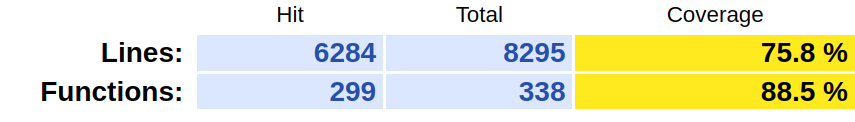
\includegraphics[scale=0.5]{cover2.png}
	\caption{Расширенное покрытие}
	\label{cover2}
\end{figure}

По сравнению с первым экспериментом тестовое покрытие увеличилось на 11.8\% или на 1275 строк кода.

\subsection{Фаззинг-тестирование}

Наиболее популярный инструмент фаззинг-тестирования ядра Linux и его модулей - syzkaller. Однако он плохо подходит для задачи тестирования файловой системы, так как суть его работы заключается в генерации случайных программ состоящих из различных системных вызовов. Для достижения типичного сценария работы ФС syzkaller должен сгенерировать программу, состоящую как минимум из монтирования валидного образа файловой системы и дальнейших взаимодействий с ним при помощи, например, системных вызовов open, write и close. Для случайной генерации подходящего сценария потребуется множество перебранных неудачных вариантов последовательностей системных вызовов или монтирования невалидных образов.

Для того, чтобы сузить тестируемые syzkaller области, был применен файл конфигурации, приведенный в приложении (А). Параметры конфигурации syzkaller указывают ему список разрешенных к использованию системных вызовов и запрещают другие, чтобы он быстрее приходил к нужному сценарию. Инструменты описания грамматики системных вызовов, разработанные в syzkaller позволяют определить свою "мутацию" системного вызова заключающуюся, например, в определенных передаваемых параметрах. Таким образом в файле sys/linux/filesystem.txt определен системный вызов монтирования образа файловой системы JFFS2: "syz\_mount\ \_image\$jffs2". При включении этого вызова в конфигурации и отключении других вариантов монтирования, монтирование всего будет производиться с параметром типа файловой системы jffs2.

При столкновении с ошибкой в виде блокировки, неопределенного поведения, либо просто сообщения об ошибке или предупреждения syzkaller генерирует программу репродьюсер на языке C, при запуске которой будет воспроизведен сценарий достигающий этой ошибки. Для генерации репродьюсеров при достижении определенной строки нужно добавить в коде ядра генерацию предупреждения об ошибке при достижении этой строки, что можно реализовать, например, при помощи макроса "WARN\_ON(1)".

При помощи syzkaller удалось достичь покрытия 11 ранее непокрытых строк, отвечающих редким сценариям при обработке суперблока в процессе монтировании ФС.

Таким образом для расширения покрытия кода ФС, syzkaller был запущен в конфигурации, разрешающей ему производить только системные вызовы для работы с ФС. Достигаемое им тестовое покрытие было проанализировано и в недостижимые ранее строки были помещены предупреждения об ошибках. При повторном запуске syzkaller при достижении этих строк он генерировал программы репродьюсеры, которые необходимо добавить в разрабатываемую систему автоматизированного тестирования.

На рис. ~\ref{covers1} продемонстрировано покрытие до запуска программ репродьюсеров, на рис. ~\ref{covers2} ~--- покрытие после их запуска.

\begin{figure}[H]
	\centering
	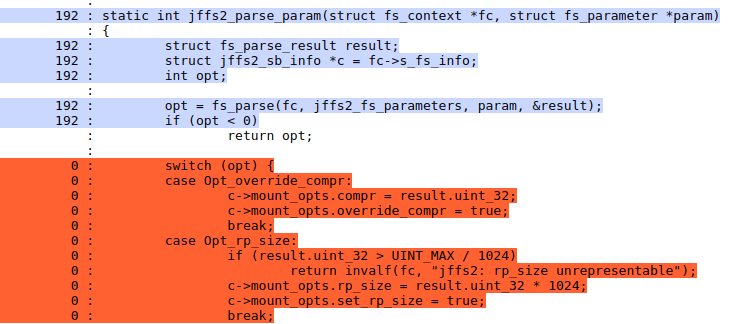
\includegraphics[scale=0.5]{covers1.png}
	\caption{Покрытие без фаззинга}
	\label{covers1}
\end{figure}

\begin{figure}[H]
	\centering
	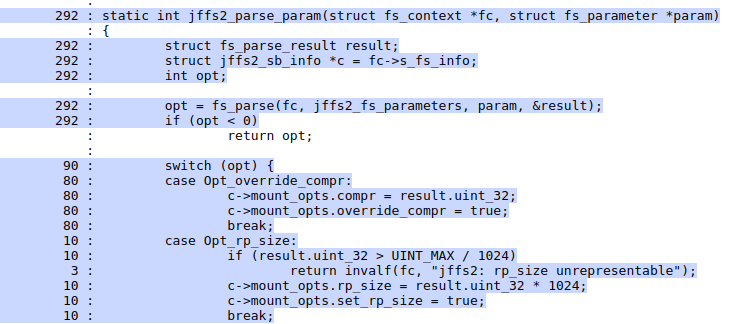
\includegraphics[scale=0.5]{covers2.png}
	\caption{Покрытие с применением фаззинга}
	\label{covers2}
\end{figure}

При тестировании JFFS2 при помощи доработанного инструмента фаззинга файловых систем fsfuzz было также достигнуто покрытие 13 ранее непокрытых строк, составляющих две ранее непокрытые функции обновления опций монтирования при реконфигурации суперблока ФС.

Таким образом, фаззинг-тестирование помогло покрыть 24 ранее непокрытых строки кода, достижимые только при редких случаях работы ФС.

\subsection{Тестирование с использованием симуляции сбоев}

Исходном код модулей ядра Linux и ФС в частности содержат множество строк кода, отвечающих за обработку крайне редко происходящих сценариев, которые однако в случае возникновения должны быть корректно обработаны. Наглядным примером подобных обработчиков ошибок, редко встречаемых в типичном сценарии работы модуля, является проверка значения, возвращаемого функциями выделения памяти. Для тестирования корректной работы ядра в подобном сценарии используется технология симуляции сбоев \cite{faultuse}.

В данной работе применялся метод целенаправленной разработки тестов с симуляцией сбоев, который малоэффективен при создании универсальной системы тестирования нескольких модулей или драйверов ядра, однако подходит для создания тестов направленных на работу с определенной файловой системой.

При анализе тестового покрытия был обнаружен достаточно большой участок кода, обрабатывающий сценарий сбоя в функции записи данных на флэш-память jffs2\_flash\_writev. Соседние этому обработчику ошибки строки покрываются тестом номер 3 из группы generic из набора xfstests. 

Для симуляции сбоя в этой функции был использован инструмент Linux Fault Injection, функционал которого можно подключить, определив в файле конфигурации ядра параметр "CONFIG\_FAULT\_INJECTION".\ В параметрах внедрения ошибок было указано имя функции, в которой по тестовому сценарию должен произойти сбой, единичный интервал между сбоями, вероятность сбоя 100\%, количество сбоев равное количеству запуска тестируемой функции в рассматриваемом тесте набора и возвращаемое значение функции -12, соответствующее коду ошибки в случае отсутствия свободной памяти (-ENOMEM). Покрытие участка кода обработчика ошибок до тестирования с использованием симуляции сбоя приведено на рис. ~\ref{coverf1}.

\begin{figure}[H]
	\centering
	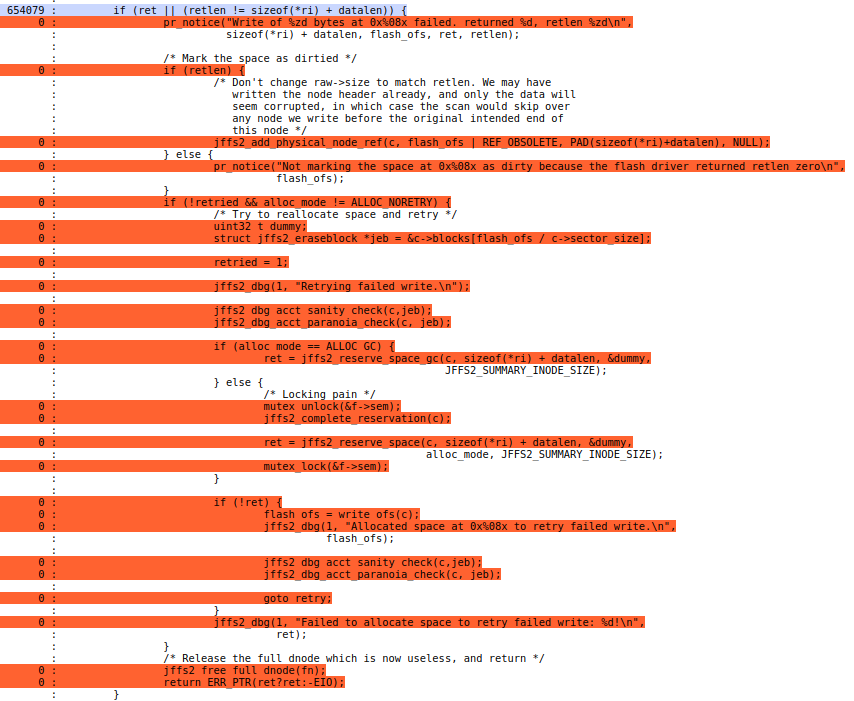
\includegraphics[scale=0.5]{coverf1.png}
	\caption{Покрытие без симуляции сбоев}
	\label{coverf1}
\end{figure}

При запуске выбранного теста с использованием симуляции сбоя функции jffs2\_flash\_writev удалось покрыть 24 ранее непокрытые строки обработки ошибки в запускающей ее функции jffs2\_write\_dnode, а также ранее непокрытую функцию проверки корректности суперблока ФС в случае подобной ошибки, состоящую из 5 строк кода. Кроме того дополнительно были покрыты 7 строк обрабатывающие ошибку произошедшую в функции jffs2\_write\_dnode. Таким образом тест с использованием симуляции сбоя во внутренней функции JFFS2 покрывает 36 ранее непокрытых строк. Покрытие того же участка кода, после включения в систему нового теста приведено на рис. ~\ref{coverf2}.

\begin{figure}[H]
	\centering
	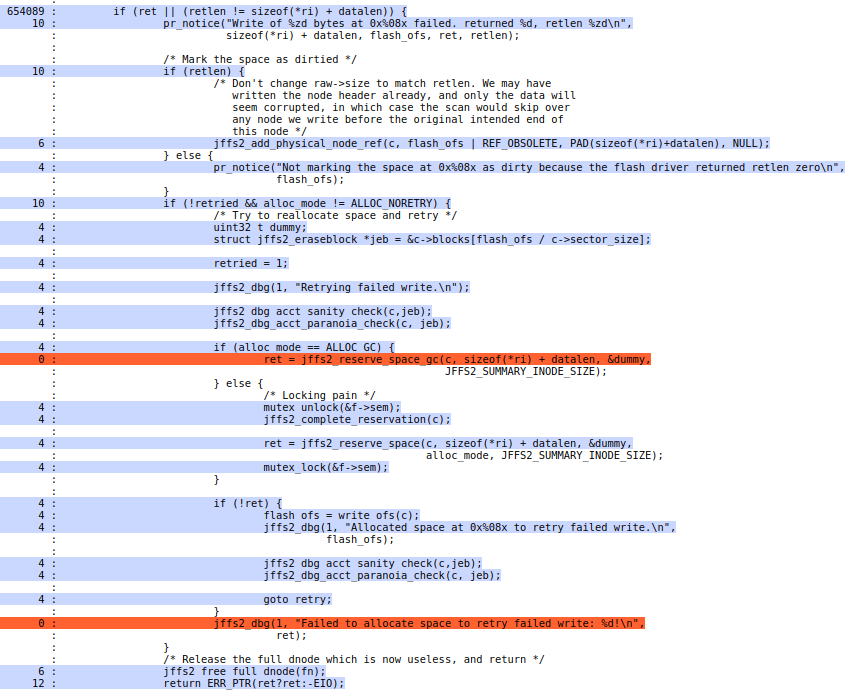
\includegraphics[scale=0.5]{coverf2.png}
	\caption{Покрытие с применением симуляции сбоев}
	\label{coverf2}
\end{figure}

Аналогичным образом был создан второй тест, на основе того же теста из набора xfstests, покрывающий при помощи симуляции ошибки в функции создания нового индексного дескриптора по причине нехватки памяти. Данный тест покрывает 3 новые строки кода функции jffs2\_create.

\subsection{Анализ непокрытого кода}

Суммарное покрытие, достигаемое тестами из набора xfstests и пакета mtd-utils, тестами, созданными из программ репродьюсеров сгенерированных инструментом syzkaller и фаззинг-тестирования при помощи fsfuzz составляет 6216 строк кода из 7829, что соответствует покрытию 79.4\% строк исходного кода. Функциональное покрытие составляет 91.4\% или 286 из 313 функций. Визуализация итоговой информации о покрытии, собранной утилитой lcov представлена на рис. ~\ref{final}.

\begin{figure}[H]
	\centering
	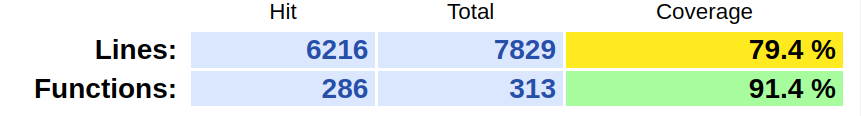
\includegraphics[scale=0.5]{final.png}
	\caption{Покрытие достигаемое разработанной системой}
	\label{final}
\end{figure}

При достижении подобного результата дальнейшее увеличение тестового покрытия кода является крайне трудоёмкой задачей и покрытие 79.4\% строк кода можно считать достойным результатом. Однако каждая функция добавляется в код ФС для выполнения особой задачи, и факт наличия непокрытых функций является проблемой, так как тестовые скрипты не соответствуют всем возможным сценариям работы файловой системы.

Для дальнейшего развития системы тестирования исследуемой файловой системы и подведения итогов проделанной работы необходимо провести анализ непокрытого кода.

Оставшиеся непокрытыми 27 функций были классифицированы на 4 группы. Результат представлен на рис. ~\ref{funcs}.

\begin{figure}[H]
	\centering
	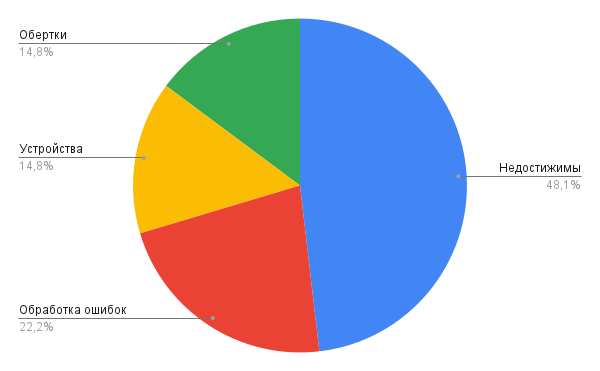
\includegraphics[scale=0.75]{chart.png}
	\caption{Катеогории непокрытых функций}
	\label{funcs}
\end{figure}

Во-первых, 13 из этих функций можно считать недостижимыми при подходе тестирования скриптами пространства пользователя. Наглядным примером являются функции деинициализации алгоритмов сжатия. Деинициализация структур, хранящих данные об алгоритмах сжатия, происходит в случае возникновении ошибки при инициализации модуля ФС, что происходит на этапе загрузки ядра ОС. Внедрить ошибки для тестирования подобного сценария невозможно используя скрипты пространства пользователя.

Во-вторых, 6 функций отвечают за обработку ошибок в редких сценариях и могут быть покрыты при помощи специальных тестов с использованием симуляции сбоев, аналогично тестам, описанным в прошлом разделе.

В-третьих, 4 непокрытых функций нужны для работы ФС с особыми видами устройств флэш-памяти. Например, функция jffs2\_dataflash\_setup и jffs2\_dataflash\_cleanup выполняют соответственно инициализацию и деинициализацию буфера записи, для работы с устройством dataflash. Еще 2 функции имеют такое же назначение, но для работы с NOR-памятью с контроллером.

В-четвертых, 4 функции отвечают за операции с суперблоком файловой системы, как, например, поиск родительского каталога. Эти функции могут быть покрыты тестами пользовательского пространства, однако они фактически являются обертками над функциями, которые являются общими для всех ФС и определены вне директории модуля JFFS2. Как, например, функция jffs2\_fh\_to\_parent просто ссылается на функцию generic\_fh\_to\_parent, определенную в файле fs/libfs.c.

\newpage
